\documentclass[12pt, twoside]{article}
\input{../preamble}

\fancyhead[LE]{\thepage}
\fancyhead[RO]{\thepage}
\fancyhead[LO]{La Scuola d'Italia / Dr.\ Huson / IB Math --- Solutions \\* 7 March 2026}

\begin{document}
\subsubsection*{5.1 Classwork: Introduction to Kinematics --- Solutions}

\begin{enumerate}[itemsep=0.15cm]

%--- Problem 1 ---
\item A runner jogs 400\,m east and then 150\,m west.
\begin{enumerate}[itemsep=0.1cm]
  \item Find the total \textbf{distance} the runner travels. \hfill [1]
  \item Find the runner's \textbf{displacement} from the starting point.
        State the direction. \hfill [2]
  \item Explain why these two answers are different. \hfill [1]
\end{enumerate}

\vfill

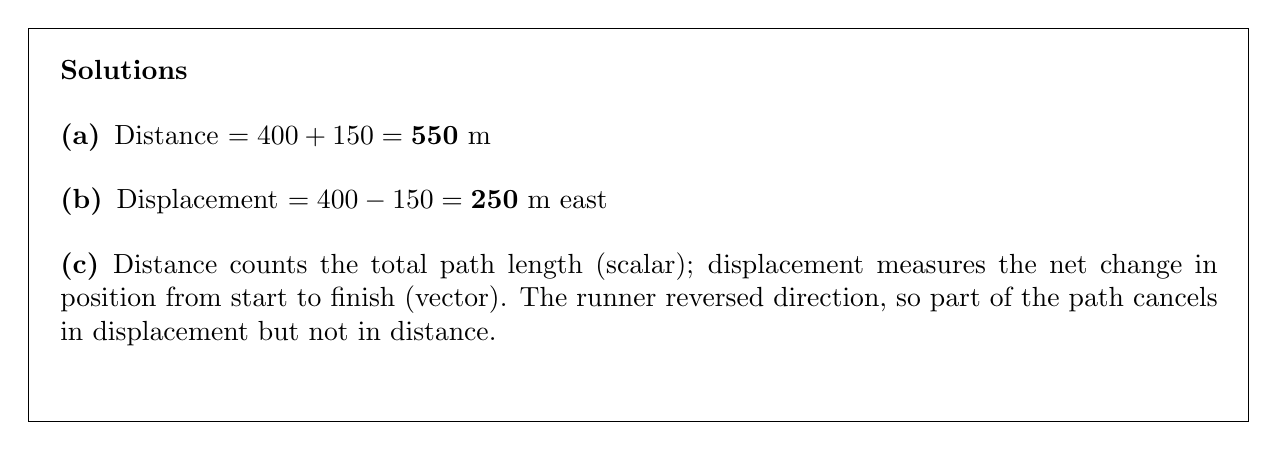
\begin{tikzpicture}
  \draw (0,0) rectangle (15.5,5);
  \node[anchor=north west, inner sep=0.40cm] at (0,5) {%
    \begin{minipage}[t]{14.7cm}%
      \textbf{Solutions}\\[0.4cm]
      \textbf{(a)}\enspace Distance $= 400 + 150 = \mathbf{550}$ m\\[0.4cm]
      \textbf{(b)}\enspace Displacement $= 400 - 150 = \mathbf{250}$ m east\\[0.4cm]
      \textbf{(c)}\enspace Distance counts the total path length (scalar); displacement
      measures the net change in position from start to finish (vector). The runner
      reversed direction, so part of the path cancels in displacement but not in distance.%
    \end{minipage}%
  };
\end{tikzpicture}

%--- Problem 2 ---
\item The graph below shows the position $s$ (metres) of a particle
      at time $t$ (seconds).

\begin{center}
\vspace{-0.3cm}
\begin{tikzpicture}[scale=0.6]
  \draw[-{Stealth}] (-0.5,0) -- (9,0) node[right] {$t$ (s)};
  \draw[-{Stealth}] (0,-2.5) -- (0,5.5) node[above] {$s$ (m)};
  \foreach \x in {1,...,8} \draw[gray!30] (\x,-2.5)--(\x,5.5);
  \foreach \y in {-2,...,5} \draw[gray!30] (-0.5,\y)--(9,\y);
  \foreach \x in {1,2,...,8} \draw (\x,0.1)--(\x,-0.1) node[below]{\small\x};
  \foreach \y in {-2,-1,1,2,3,4,5} \draw (0.1,\y)--(-0.1,\y) node[left]{\small\y};
  \node[below left] at (0,0) {\small 0};
  \draw[very thick]
    (0,0) -- (2,4) -- (5,4) -- (7,-2) -- (8,-2);
  \foreach \pt in {(0,0),(2,4),(5,4),(7,-2),(8,-2)}
    \fill \pt circle (2.5pt);
\end{tikzpicture}
\vspace{-0.3cm}
\end{center}

\begin{enumerate}[itemsep=0.1cm]
  \item Find the velocity of the particle during $0 \leq t \leq 2$. \hfill [2]
  \item Describe the motion of the particle during $2 \leq t \leq 5$. \hfill [1]
  \item Find the velocity during $5 \leq t \leq 7$. \hfill [2]
  \item Find the total \textbf{distance} travelled from $t=0$ to $t=7$. \hfill [2]
  \item Find the \textbf{displacement} from $t=0$ to $t=7$. \hfill [1]
\end{enumerate}

\vfill

\begin{tikzpicture}
  \draw (0,0) rectangle (15.5,7);
  \node[anchor=north west, inner sep=0.40cm] at (0,7) {%
    \begin{minipage}[t]{14.7cm}%
      \textbf{Solutions}\\[0.4cm]
      \textbf{(a)}\enspace $v = \dfrac{\Delta s}{\Delta t} = \dfrac{4 - 0}{2 - 0}
        = \mathbf{2}$ m\,s$^{-1}$\\[0.4cm]
      \textbf{(b)}\enspace The particle is stationary (displacement is constant at 4\,m).\\[0.4cm]
      \textbf{(c)}\enspace $v = \dfrac{-2 - 4}{7 - 5} = \dfrac{-6}{2}
        = \mathbf{-3}$ m\,s$^{-1}$\\[0.4cm]
      \textbf{(d)}\enspace Distance $= |4 - 0| + |4 - 4| + |-2 - 4| = 4 + 0 + 6
        = \mathbf{10}$ m\\[0.4cm]
      \textbf{(e)}\enspace Displacement $= s(7) - s(0) = -2 - 0 = \mathbf{-2}$ m%
    \end{minipage}%
  };
\end{tikzpicture}

\newpage

%--- Problem 3 ---
\item The velocity $v$ (m\,s$^{-1}$) of a particle is shown below.

\begin{center}
\vspace{-0.3cm}
\begin{tikzpicture}[scale=0.6]
  \draw[-{Stealth}] (-0.5,0) -- (9,0) node[right] {$t$ (s)};
  \draw[-{Stealth}] (0,-1.5) -- (0,5.5) node[above] {$v$ (m\,s$^{-1}$)};
  \foreach \x in {1,...,8} \draw[gray!30] (\x,-1.5)--(\x,5.5);
  \foreach \y in {-1,...,5} \draw[gray!30] (-0.5,\y)--(9,\y);
  \foreach \x in {1,2,...,8} \draw (\x,0.1)--(\x,-0.1) node[below]{\small\x};
  \foreach \y in {-1,1,2,3,4,5} \draw (0.1,\y)--(-0.1,\y) node[left]{\small\y};
  \node[below left] at (0,0) {\small 0};
  \draw[very thick]
    (0,0) -- (3,3) -- (6,3) -- (8,0);
  \foreach \pt in {(0,0),(3,3),(6,3),(8,0)}
    \fill \pt circle (2.5pt);
\end{tikzpicture}
\vspace{-0.3cm}
\end{center}

\begin{enumerate}[itemsep=0.1cm]
  \item Find the acceleration during $0 \leq t \leq 3$. \hfill [2]
  \item State the acceleration during $3 \leq t \leq 6$. \hfill [1]
  \item Find the acceleration during $6 \leq t \leq 8$. \hfill [2]
  \item Is the particle slowing down during $6 \leq t \leq 8$?
        Explain your answer. \hfill [1]
\end{enumerate}

\vfill

\begin{tikzpicture}
  \draw (0,0) rectangle (15.5,7);
  \node[anchor=north west, inner sep=0.40cm] at (0,7) {%
    \begin{minipage}[t]{14.7cm}%
      \textbf{Solutions}\\[0.4cm]
      \textbf{(a)}\enspace $a = \dfrac{\Delta v}{\Delta t} = \dfrac{3 - 0}{3 - 0}
        = \mathbf{1}$ m\,s$^{-2}$\\[0.4cm]
      \textbf{(b)}\enspace $a = \mathbf{0}$ m\,s$^{-2}$ (constant velocity)\\[0.4cm]
      \textbf{(c)}\enspace $a = \dfrac{0 - 3}{8 - 6} = \dfrac{-3}{2}
        = \mathbf{-1.5}$ m\,s$^{-2}$\\[0.4cm]
      \textbf{(d)}\enspace Yes. The velocity is positive but decreasing toward zero, so the
      particle is moving forward but slowing down (decelerating).%
    \end{minipage}%
  };
\end{tikzpicture}

%--- Problems 4, 5, 6, 7 ---
\item Scalar or vector. \hfill [4]

\item Negative velocity at $t = 4$.

\item Position table: $s = 2, 5, 8, 11, 14$.

\item Cyclist from rest, $a = 2$\,m\,s$^{-2}$ for 5 seconds.

\vfill

\begin{tikzpicture}
  \draw (0,0) rectangle (15.5,11);
  \node[anchor=north west, inner sep=0.40cm] at (0,11) {%
    \begin{minipage}[t]{14.7cm}%
      \textbf{Solutions to Problems 4--7}\\[0.4cm]
      \textbf{Problem 4:}\enspace
        (a) Scalar (speed, no direction given)\\[0.1cm]
      \hspace*{2.5em}(b) Vector (displacement, direction north)\\[0.1cm]
      \hspace*{2.5em}(c) Vector (velocity, has sign)\\[0.1cm]
      \hspace*{2.5em}(d) Scalar (temperature)\\[0.5cm]
      \textbf{Problem 5:}\\[0.2cm]
      \textbf{(a)}\enspace The negative sign means the particle is moving in the negative
      direction (to the left).\\[0.2cm]
      \textbf{(b)}\enspace Speed $= |v| = |-3| = \mathbf{3}$ m\,s$^{-1}$\\[0.5cm]
      \textbf{Problem 6:}\\[0.2cm]
      \textbf{(a)}\enspace $v = \dfrac{\Delta s}{\Delta t} = \dfrac{5 - 2}{1 - 0}
        = \mathbf{3}$ m\,s$^{-1}$ (constant, same for every interval)\\[0.4cm]
      \textbf{(b)}\enspace $a = \mathbf{0}$ m\,s$^{-2}$ (velocity is constant)\\[0.2cm]
      \textbf{(c)}\enspace The particle moves at a constant velocity of 3\,m\,s$^{-1}$
      in the positive direction (uniform motion, no acceleration).\\[0.5cm]
      \textbf{Problem 7:}\\[0.2cm]
      \textbf{(a)}\enspace $v = u + at = 0 + 2 \times 5 = \mathbf{10}$ m\,s$^{-1}$\\[0.2cm]
      \textbf{(b)}\enspace Straight line from $(0, 0)$ to $(5, 10)$ on the $v$--$t$ graph.%
    \end{minipage}%
  };
\end{tikzpicture}

\end{enumerate}
\end{document}
